\documentclass[11pt,a4paper]{article}
\usepackage[utf8]{inputenc}
\usepackage[T1]{fontenc}
\usepackage[brazil]{babel}
\usepackage{lmodern}
\usepackage[margin=2cm]{geometry}
\usepackage{amsmath,amssymb}
\usepackage{booktabs}
\usepackage{graphicx}
\usepackage{hyperref}
\usepackage{xcolor}
\usepackage{titlesec}
\usepackage{tabularx}
\usepackage{enumitem}
\usepackage{float}
\usepackage{array}
\renewcommand{\tabularxcolumn}[1]{>{\raggedright\arraybackslash}p{#1}}
\usepackage{newunicodechar}
\usepackage[most]{tcolorbox}
\usepackage{etoolbox}

\hypersetup{colorlinks=true, linkcolor=blue!70!black, citecolor=blue!70!black, urlcolor=blue!70!black}

\titleformat{\section}{\large\bfseries}{\thesection.}{0.5em}{}
\titleformat{\subsection}{\normalsize\bfseries}{\thesubsection.}{0.5em}{}
\titlespacing*{\section}{0pt}{1.2ex plus 0.5ex minus .2ex}{0.6ex}
\titlespacing*{\subsection}{0pt}{1.0ex plus 0.4ex minus .2ex}{0.4ex}
\setlength{\parskip}{0.45em}
\setlength{\parindent}{0pt}
\setlist{itemsep=0.15em,topsep=0.3em}

% --- símbolos ---
\newunicodechar{π}{\ensuremath{\pi}}
\newunicodechar{τ}{\ensuremath{\tau}}
\newunicodechar{φ}{\ensuremath{\varphi}}
\newunicodechar{ψ}{\ensuremath{\psi}}
\newunicodechar{Σ}{\ensuremath{\Sigma}}
\newunicodechar{→}{\ensuremath{\rightarrow}}
\newunicodechar{⇒}{\ensuremath{\Rightarrow}}
\newunicodechar{∈}{\ensuremath{\in}}
\newunicodechar{−}{\ensuremath{-}}
\newunicodechar{≈}{\ensuremath{\approx}}
\newunicodechar{≠}{\ensuremath{\neq}}
\newunicodechar{≡}{\ensuremath{\equiv}}
\newunicodechar{≤}{\ensuremath{\leq}}
\newunicodechar{≥}{\ensuremath{\geq}}
\newunicodechar{′}{\ensuremath{'}}
\newunicodechar{‑}{-}
\newunicodechar{✔}{\ensuremath{\checkmark}}
\newunicodechar{✘}{\ensuremath{\times}}

% --- cores e caixas ---
\definecolor{cC}{HTML}{7A4FA3}
\definecolor{cS}{HTML}{2F7D74}
\definecolor{cAcc}{HTML}{2F5D8A}
\newcommand{\metrictag}[2]{{\setlength{\fboxsep}{1.5pt}%
  \ifstrequal{#1}{c}{\colorbox{cC}{\textcolor{white}{\scriptsize\textbf{#2}}}}{%
  \ifstrequal{#1}{s}{\colorbox{cS}{\textcolor{white}{\scriptsize\textbf{#2}}}}{%
  \colorbox{black!60}{\textcolor{white}{\scriptsize\textbf{#2}}}}}}}
\newcommand{\pagechip}[1]{{\setlength{\fboxsep}{1.5pt}\colorbox{cAcc}{\textcolor{white}{\scriptsize\texttt{#1}}}}}
\newcommand{\readtag}[1]{\texttt{\small #1}}
\newcommand{\partbar}[1]{\par\vspace{1.2em}\noindent\colorbox{black!80}{\parbox{\dimexpr\linewidth-2\fboxsep}{\color{white}\bfseries\sffamily\MakeUppercase{#1}}}\par\vspace{0.4em}}
\newtcolorbox{citacard}[1]{breakable, enhanced, colback=white, colframe=black!25, boxrule=0.5pt, arc=2pt,
  left=6pt, right=6pt, top=4pt, bottom=4pt, title={\small #1}, coltitle=black, colbacktitle=black!6, fonttitle=\normalfont}
\newenvironment{origquote}{\par\itshape\small}{\par}
\newenvironment{tradquote}{\par\small\textsc{Tradução:}\ }{\par}
\newcommand{\explab}[1]{\par\smallskip{\small\color{cAcc}\textbf{\MakeUppercase{#1}}}\par}
\colorlet{notebg}{blue!4}\colorlet{notefg}{cAcc}
\colorlet{okbg}{green!5}\colorlet{okfg}{green!45!black}
\colorlet{warnbg}{orange!8}\colorlet{warnfg}{orange!80!black}
\newtcolorbox{infobox}[2][note]{breakable, enhanced, boxrule=0pt, arc=2pt, left=6pt, right=6pt, top=4pt, bottom=4pt,
  colback=#1bg, borderline west={3pt}{0pt}{#1fg}, frame hidden,
  before upper={\ifstrempty{#2}{}{\textbf{#2}\par}}}
\colorlet{pairc}{cC}\colorlet{pairs}{cS}
\newenvironment{paircol}[2]{\begin{tcolorbox}[width=0.485\linewidth, nobeforeafter, box align=top, boxrule=0.5pt,
  colframe=black!25, colback=white, borderline north={3pt}{0pt}{pair#1}, left=5pt, right=5pt,
  before upper={{\color{pair#1}\small\textbf{\MakeUppercase{#2}}}\par}]}{\end{tcolorbox}}

\begin{document}

\begin{center}
    {\LARGE \textbf{Fichamento: Consistency e Sufficiency}} \\[0.35em]
    {\large DASGUPTA, S.; FROST, N.; MOSHKOVITZ, M. \textit{Framework for Evaluating Faithfulness of Local Explanations}. ICML, 2022, p.~4794--4815 (arXiv:2202.00734v1)} \\[0.3em]
    \textbf{Aluno:} Arthur Santos de Oliveira (RA: 156297) \\[0.2em]
    \textbf{Atualizado em:} 09/10/2026 \\[0.2em]
    \textbf{Repositório:} \url{https://github.com/Arthur-so/shap-ecg-arrhythmia}
\end{center}
\vspace{-0.5em}
\hrule
\vspace{0.8em}

\textbf{Como ler.} \texttt{[p. N]} indica a página do PDF do artigo. As citações estão no original em inglês, cada uma seguida de uma tradução livre. A \textbf{Parte I} explica as duas métricas sem pressupor a leitura do artigo; a \textbf{Parte II} é o fichamento, em ordem de páginas, com cada citação marcada pela métrica a que se refere (\metrictag{c}{C} Consistency, \metrictag{s}{S} Sufficiency, \metrictag{cs}{C + S} as duas); a \textbf{Parte III} relaciona o artigo ao TCC, com as decisões tomadas e os resultados atuais.


\partbar{Parte I · Entendendo as métricas}

\section{O problema que o artigo resolve}
Um modelo faz uma \textbf{predição} (“este ECG é STE”) e um método como o SHAP gera uma \textbf{explicação} (“olhei principalmente para estes trechos”). A pergunta do artigo é simples: \textbf{essa explicação é honesta?} Ela descreve de verdade o motivo da decisão do modelo, ou só parece convincente?

Os autores chamam isso de \textit{fidelidade} (\textit{faithfulness}) e propõem \textbf{duas medidas complementares}: \textbf{Consistency} e \textbf{Sufficiency}. As duas usam a mesma lógica (“exemplos parecidos do ponto de vista da explicação devem receber a mesma resposta do modelo”) e diferem só em \textbf{quem conta como parecido}.

\section{Consistency e Sufficiency lado a lado}
O exemplo é dos próprios autores \texttt{[p. 3]}. Um modelo olha fotos de paisagens e diz o bioma. Um \textbf{explicador} (no seu caso, o SHAP) diz, para cada foto, \textbf{o que fez o modelo responder aquilo}. Imagine 4 fotos:

\begin{center}\small
\begin{tabularx}{\linewidth}{XXXX}
\toprule
\textbf{Foto} & \textbf{O que aparece na foto} & \textbf{O que o explicador disse} & \textbf{Resposta do modelo} \\
\midrule
\textbf{1} & zebra no capim & “foi por causa da \textbf{zebra}” & savana \\
2 & zebra no capim & “foi por causa da \textbf{zebra}” & savana \\
3 & zebra num zoológico, com prédios ao fundo & “foi por causa dos \textbf{prédios}” & cidade \\
4 & leão no capim & “foi por causa do \textbf{leão}” & savana \\
\bottomrule
\end{tabularx}
\end{center}

Vamos avaliar a \textbf{foto 1}. A explicação dela é “zebra”. As duas métricas escolhem de jeitos diferentes \textbf{com quais outras fotos comparar}:

\noindent
\begin{paircol}{c}{Consistency}
\textbf{Com quem comparo?} Com as fotos em que o \textbf{explicador disse a mesma coisa} (“zebra”). Olho para a \textbf{coluna “o que o explicador disse”}.

→ Só a \textbf{foto 2}. A foto 3 tem zebra, mas o explicador falou “prédios”, então fica de fora.

\textbf{A resposta é a mesma?} Foto 2 = savana ✔ → \textbf{1/1 = 1,0}
\end{paircol}
\hfill
\begin{paircol}{s}{Sufficiency}
\textbf{Com quem comparo?} Pego a \textbf{explicação da foto 1} (“zebra”) e procuro essa coisa nas outras fotos: entram as fotos em que \textbf{a zebra aparece}, não importa o que o explicador disse \textit{sobre elas}. Uso a explicação da foto 1 e a \textbf{coluna “o que aparece na foto”} das outras.

→ \textbf{Fotos 2 e 3}. A foto 3 entra porque tem zebra.

\textbf{A resposta é a mesma?} Foto 2 = savana ✔, foto 3 = cidade ✘ → \textbf{1/2 = 0,5}
\end{paircol}

\begin{infobox}[ok]{A diferença numa frase}
A \textbf{Consistency} pergunta: \textit{“quando o explicador dá a mesma justificativa, o modelo dá a mesma resposta?”} Ela compara a explicação da foto 1 com as \textbf{explicações} das outras fotos.\newline  A \textbf{Sufficiency} pergunta: \textit{“onde quer que a coisa apontada pela explicação apareça, o modelo dá a mesma resposta?”} Ela parte da \textbf{explicação} da foto 1 (é ela que diz o que procurar) e procura isso no \textbf{conteúdo} das outras fotos.\newline \newline  No exemplo, a Consistency deu 1,0 porque toda vez que o explicador disse “zebra” o modelo disse savana. A Sufficiency deu 0,5 porque revelou um problema: existe uma foto com zebra (a 3) em que o modelo \textbf{não} disse savana. Ou seja, “ter zebra” \textbf{não é suficiente} para o modelo responder savana, e a explicação da foto 1 era incompleta.
\end{infobox}

\begin{infobox}[warn]{As duas usam a explicação. Nenhuma olha só para a entrada.}
É fácil ler a Sufficiency como “fotos parecidas recebem a mesma resposta?”, mas não é isso. Sem a explicação da foto 1, ela nem saberia \textbf{o que procurar} nas outras fotos. O que muda entre as duas é \textbf{quais explicações} entram na conta:

\begin{center}\small
\begin{tabularx}{\linewidth}{XXXX}
\toprule
 & \textbf{Explicação da foto analisada} & \textbf{Explicações das outras fotos} & \textbf{Conteúdo das outras fotos} \\
\midrule
\metrictag{c}{C} Consistency & \textbf{usa} (“zebra”) & \textbf{usa} (quem também recebeu “zebra”?) & não usa \\
\metrictag{s}{S} Sufficiency & \textbf{usa} (“zebra” = o que procurar) & ignora & \textbf{usa} (quem tem zebra?) \\
\bottomrule
\end{tabularx}
\end{center}

Comparar só as entradas (“fotos parecidas → mesma resposta?”) mediria outra coisa: a estabilidade do \textbf{modelo}, sem envolver explicação nenhuma. Não é o que nenhuma das duas faz.
\end{infobox}

\subsection{A conta de cada uma, passo a passo}
As duas fazem a \textbf{mesma sequência de passos}. Só o passo 2 (quem entra no grupo) muda. Seguindo com a foto 1 do exemplo acima:

\begin{center}\small
\begin{tabularx}{\linewidth}{lXX}
\toprule
\textbf{Passo} & \textbf{\metrictag{c}{C} Consistency} & \textbf{\metrictag{s}{S} Sufficiency} \\
\midrule
\textbf{1.} Escolho uma foto & \multicolumn{2}{>{\hsize=\dimexpr2\hsize+2\tabcolsep\relax}X}{Foto 1: explicação “zebra”, resposta “savana”.} \\
\textbf{2.} Monto o grupo de comparação & Outras fotos em que o \textbf{explicador também disse “zebra”} → foto 2 & Uso a explicação da foto 1 (“zebra”) como o que procurar: outras fotos em que \textbf{aparece uma zebra} → fotos 2 e 3 \\
\textbf{3.} Conto quantas do grupo têm a mesma resposta (“savana”) & Foto 2 = savana → \textbf{1 de 1} & Foto 2 = savana, foto 3 = cidade → \textbf{1 de 2} \\
\textbf{4.} Divido: escore da foto 1 & 1 ÷ 1 = \textbf{1,0} & 1 ÷ 2 = \textbf{0,5} \\
\bottomrule
\end{tabularx}
\end{center}

\textbf{Passo 5: repito para todas as fotos e tiro a média.} Esse é o escore final da métrica:

\begin{center}\small
\begin{tabularx}{\linewidth}{XXXX}
\toprule
\textbf{Foto} & \textbf{Explicação} & \textbf{\metrictag{c}{C} grupo → escore} & \textbf{\metrictag{s}{S} grupo → escore} \\
\midrule
1 & zebra & \{2\} → 1/1 = 1,0 & \{2, 3\} → 1/2 = 0,5 \\
2 & zebra & \{1\} → 1/1 = 1,0 & \{1, 3\} → 1/2 = 0,5 \\
3 & prédios & ninguém mais com “prédios” → \textbf{0} & nenhuma outra foto tem prédios → \textbf{0} \\
4 & leão & ninguém mais com “leão” → \textbf{0} & nenhuma outra foto tem leão → \textbf{0} \\
\multicolumn{2}{>{\hsize=\dimexpr2\hsize+2\tabcolsep\relax}X}{\textbf{Média (escore final)}} & \textbf{(1 + 1 + 0 + 0) / 4 = 0,50} & \textbf{(0,5 + 0,5 + 0 + 0) / 4 = 0,25} \\
\bottomrule
\end{tabularx}
\end{center}

Repare nas fotos 3 e 4: como não há com quem compará-las, elas entram com \textbf{0}. É assim que o artigo \texttt{[p. 11]} e o Quantus fazem: sem evidência, a foto conta como “não fiel”. Isso puxa as duas médias para baixo, e voltaremos a esse ponto na seção 4.1.

O escore vai de 0 a 1, e maior é melhor. Perto de 1: a explicação permite prever o que o modelo responde. Perto de 0: o modelo responde coisas diferentes para fotos “parecidas” do ponto de vista da explicação, ou não há fotos parecidas para comparar.

\begin{infobox}[warn]{Detalhe importante: nenhuma das duas usa o gabarito}
No passo 3, verifica-se se o \textbf{modelo respondeu} “savana”, e não se a foto \textbf{é de fato} uma savana. Por exemplo, se uma das fotos com zebra fosse de um zoológico e o modelo dissesse “savana”, ela \textbf{contaria a favor}: o modelo errou, mas foi coerente com a explicação que deu.\newline \newline  Isso é proposital. As duas métricas não medem se o modelo acerta (isso é o F1). Elas medem se a explicação \textbf{descreve com honestidade o comportamento do modelo}, mesmo quando ele erra. No seu ECG, o diagnóstico do cardiologista não entra na conta, só a classe que o \textbf{modelo} deu. (Há uma ressalva sobre o seu pipeline na seção 11.)
\end{infobox}

\section{Traduzindo para o ECG}

No TCC, a explicação não é uma frase como “tem zebra”. É um \textbf{mapa de calor} do GradientSHAP: para cada uma das 12 derivações e cada um dos 15\,000 instantes, um número que diz o quanto aquele ponto pesou na decisão do modelo. \textbf{Mapa SHAP e explicação são a mesma coisa.} Isso cria um problema diferente para cada métrica:

\noindent
\begin{paircol}{c}{Consistency}
\textbf{Problema:} precisa de explicações \textbf{iguais}, e dois mapas de 180\,000 números nunca são idênticos.

\textbf{Solução do artigo:} \textbf{simplificar} (discretizar) o mapa antes de comparar, por exemplo guardando só os atributos mais importantes e o sinal deles \texttt{[p. 11; p. 30]}.
\end{paircol}
\hfill
\begin{paircol}{s}{Sufficiency}
\textbf{Problema:} precisa procurar a coisa apontada pela explicação \textbf{dentro} das outras entradas, como procurar a zebra numa foto. Não há como “procurar um mapa SHAP dentro de outro ECG”, e os autores admitem que não sabem resolver isso para o SHAP \texttt{[p. 8]}.
\end{paircol}

\subsection{Como o Quantus resolve}
\begin{itemize}
\item \textbf{Consistency:} simplifica cada mapa pelo sinal dos \textbf{5 primeiros} valores do vetor, depois de aplicar valor absoluto, e compara os mapas simplificados.
\item \textbf{Sufficiency:} como não dá para olhar o conteúdo dos outros ECGs, compara \textbf{mapa com mapa}: dois ECGs são “vizinhos” quando os mapas estão a uma distância pequena (até 60\% da maior distância do lote).
\item Nas duas, a predição comparada é a \textbf{classe de maior probabilidade} (top‑1), e as contas são feitas por classe, em lotes de até 64 mapas.
\end{itemize}
Os detalhes e as divergências em relação ao artigo estão na seção 7. A discretização da Consistency tinha um defeito grave, descrito na seção 9.

\subsection{Como o TCC resolve}
\begin{itemize}
\item \textbf{Sufficiency:} retirada da análise. Sem definição no artigo para mapas de importância, a versão do Quantus é, na prática, uma segunda Consistency, com tolerância de distância (seção 8).
\item \textbf{Consistency:} implementação própria, seguindo o artigo. Cada batimento é dividido em três \textbf{regiões} (pré‑QRS, QRS e ST‑T) a partir do pico R, e o mapa é resumido em 36 números (12 derivações × 3 regiões). A explicação simplificada é o conjunto das \textbf{k regiões mais importantes}, com o sinal. Todos os mapas formam uma única população, e a “predição” comparada é a \textbf{classe que o mapa explica} (seção 8).
\end{itemize}

\section{Uma conta de brinquedo no ECG}

Com o método do TCC, imagine 6 mapas SHAP, cada um explicando uma classe. Cada mapa já foi resumido na sua explicação simplificada, com k = 2 regiões:

\begin{center}\small
\begin{tabularx}{\linewidth}{lllX}
\toprule
\textbf{Mapa} & \textbf{Classe explicada} & \textbf{Explicação (k = 2)} & \textbf{Outros mapas com a mesma explicação → escore} \\
\midrule
1 & BRD & V1·QRS (+) e V2·QRS (+) & 2 (BRD), 3 (BRE) → 1/2 = 0,5 \\
2 & BRD & V1·QRS (+) e V2·QRS (+) & 1 (BRD), 3 (BRE) → 1/2 = 0,5 \\
3 & BRE & V1·QRS (+) e V2·QRS (+) & 1 (BRD), 2 (BRD) → 0/2 = 0 \\
4 & STD & II·ST‑T (+) e aVR·ST‑T (+) & 6 (STD) → 1/1 = 1 \\
5 & STE & II·pré‑QRS (+) e aVR·pré‑QRS (+) & nenhum (\textbf{sem par}) → 0 \\
6 & STD & II·ST‑T (+) e aVR·ST‑T (+) & 4 (STD) → 1/1 = 1 \\
\bottomrule
\end{tabularx}
\end{center}

Consistency por classe (média dos seus mapas): BRD = 0,5; BRE = 0; STD = 1; STE = 0. Global = (0,5 + 0,5 + 0 + 1 + 0 + 1) / 6 = \textbf{0,5}.

\subsection{O que derruba os escores}
\begin{enumerate}
\item \textbf{Classes diferentes com a mesma explicação.} O mapa 3 explica um BRE com as mesmas regiões usadas para BRD. Só pela explicação não dá para saber qual classe estava sendo justificada, e o escore cai para as duas classes.
\item \textbf{Mapa sem par vale 0.} O mapa 5 é o único com aquela explicação. Não há com quem compará-lo, e o estimador do artigo lhe atribui 0 \texttt{[p. 11]}. Isso não significa que a explicação esteja errada, só que não pôde ser verificada. Quanto maior o k, mais mapas ficam sem par.
\end{enumerate}

Diferença em relação ao Quantus: aqui não existe “classe principal”. A predição comparada é a classe que o mapa explica, e por isso a nota não cai só porque o paciente tem mais de um diagnóstico.

\begin{infobox}[ok]{Resumo da Parte I}
As duas métricas do artigo perguntam se exemplos “parecidos do ponto de vista da explicação” recebem a mesma resposta do modelo. Para mapas SHAP, só a Consistency tem uma adaptação defensável: simplificar o mapa e exigir explicações iguais. No TCC, a simplificação é feita por regiões fisiológicas do batimento, e a Sufficiency foi retirada.
\end{infobox}

\paragraph{Glossário rápido}
\begin{description}
\item[Fidelidade (faithfulness)] O quanto a explicação reflete o que o modelo realmente usa para decidir.
\item[Explicação / mapa SHAP] Saída do GradientSHAP: um número de importância para cada ponto do ECG (12 × 15000).
\item[Região] Parte de um batimento numa derivação: pré‑QRS (onda P e intervalo PR), QRS ou ST‑T. São 36 regiões (12 derivações × 3).
\item[Discretizar / simplificar] Reduzir o mapa a uma versão resumida que pode se repetir entre ECGs. No TCC: as k regiões de maior importância, com o sinal.
\item[k] Quantas regiões compõem a explicação simplificada.
\item[Sem par] Mapa cuja explicação simplificada não se repete em nenhum outro mapa. Vale 0 no estimador do artigo.
\item[Classe explicada] A classe que o mapa SHAP justifica. É a “predição” comparada na Consistency do TCC.
\item[Valor esperado ao acaso] A Consistency que se obteria se as explicações não tivessem relação com a classe. Serve só como referência.
\end{description}

\partbar{Parte II · Fichamento do artigo}

\section{Mapa de leitura}
Para entender as duas métricas e o seu caso (SHAP sobre ECG), estas partes bastam:

\begin{center}\small
\begin{tabularx}{\linewidth}{XXXX}
\toprule
\textbf{Páginas} & \textbf{Seção} & \textbf{Prioridade} & \textbf{Por quê} \\
\midrule
p. 1 & Abstract & \readtag{ler} & A tese: fidelidade = consistency + sufficiency, e as duas dependem da distribuição de teste. \\
p. 2–3 & §1.1 Contributions & \readtag{ler} & Definições intuitivas e o exemplo da zebra. \\
p. 4–6 & §2 Framework & \readtag{ler} & Definições formais 1–4. É o núcleo. \\
p. 8–9 & §3.2 Feature importance & \readtag{ler} & SHAP e gradiente; por que os autores só tratam de consistency nesses casos. \\
p. 10–11 & §4 Estimadores & \readtag{ler} & Um estimador serve para as duas; viés; explicações únicas. \\
p. 12, 14–15 & §5.1–5.2, Tab. 1–2 & \readtag{ler} & Evidência empírica: sem discretização, o escore cai para ≈ 0. \\
p. 15–16 & §5.3 & \readtag{ler} & Dependência da população: importa porque você avalia por classe. \\
p. 27 & Apêndice C & \readtag{consulta} & Algoritmo 1: estimador local das duas medidas. \\
p. 30–31 & Apêndice D.5, Tab. 5 & \readtag{ler} & Definição de “Sign-of-top-5”, a discretização que o Quantus diz usar na Consistency. \\
p. 6–7, 9–10 & §3.1, §3.3 & \readtag{pular} & Árvores, Anchors, kNN, contrafactuais: úteis só como exemplo. \\
p. 22–26, 28–29 & Apêndices A, D.1–D.4 & \readtag{pular} & Provas e detalhes de experimentos. \\
\bottomrule
\end{tabularx}
\end{center}

\section{Citações comentadas}
As citações estão em ordem de página. A etiqueta indica a métrica: \metrictag{c}{C} Consistency, \metrictag{s}{S} Sufficiency, \metrictag{cs}{C + S} as duas.

\begin{citacard}{\pagechip{p. 1} Abstract \metrictag{cs}{C + S}}
\begin{origquote}“We study the faithfulness of an explanation system to the underlying prediction model. We show that this can be captured by two properties, consistency and sufficiency, and introduce quantitative measures of the extent to which these hold. Interestingly, these measures depend on the test-time data distribution.”\end{origquote}
\begin{tradquote}“Estudamos a fidelidade de um sistema de explicação ao modelo de predição subjacente. Mostramos que ela pode ser capturada por duas propriedades, consistency e sufficiency, e introduzimos medidas quantitativas do grau em que elas se verificam. Curiosamente, essas medidas dependem da distribuição dos dados no momento do teste.”\end{tradquote}
\explab{Explicação}
Fidelidade é a propriedade geral, e Consistency e Sufficiency são as duas formas de medi-la. A última frase importa no seu caso: o valor depende de \textbf{quais exemplos} você usa para medir.
\end{citacard}

\begin{citacard}{\pagechip{p. 2} §1.1 Contributions \metrictag{cs}{C + S}}
\begin{origquote}“A prediction function (the classifier) f : X → Y […] An explanation function e : X → E, where E is the space of explanations, or properties. The explanation function explains the prediction f(x) by pointing out some relevant property of the input.”\end{origquote}
\begin{tradquote}“Uma função de predição (o classificador) f : X → Y […] Uma função de explicação e : X → E, em que E é o espaço de explicações, ou propriedades. A função de explicação explica a predição f(x) apontando alguma propriedade relevante da entrada.”\end{tradquote}
\explab{Explicação}
Todo o artigo vê o sistema como um par \textit{(f, e)}. No seu caso, \textit{f} é a ResNet34‑1D e \textit{e(x)} é o mapa GradientSHAP (12 × 15000). Para os autores, uma explicação é uma \textbf{propriedade} do exemplo (“contém uma zebra”), e não um vetor de números. É por isso que aplicar as métricas ao SHAP exige adaptações (seção 3).
\end{citacard}

\begin{citacard}{\pagechip{p. 2–3} §1.1, as duas propriedades \metrictag{cs}{C + S}}
\begin{origquote}“Consistency: Roughly, two instances x, x′ that get the same explanation should also have the same prediction. […] Sufficiency: If x is assigned an explanation e(x) = π that also holds for another instance x′ (even if e(x′) ≠ π), then x′ should have the same label as x.”\end{origquote}
\begin{tradquote}“Consistency: grosso modo, duas instâncias x, x′ que recebem a mesma explicação também deveriam ter a mesma predição. […] Sufficiency: se a x é atribuída uma explicação e(x) = π que também vale para outra instância x′ (mesmo que e(x′) ≠ π), então x′ deveria ter o mesmo rótulo que x.”\end{tradquote}
\explab{Explicação}
Este é o trecho que separa as duas. A \textbf{Consistency} compara explicação com explicação: quem recebe a \textit{mesma} explicação deve ter a mesma predição. A \textbf{Sufficiency} compara uma explicação com \textit{exemplos}: se a propriedade que justificou \textit{x} também está em \textit{x′}, a predição de \textit{x′} deve ser a mesma, \textbf{mesmo que a explicação de x′ seja outra}.

A frase do README do Quantus para a Sufficiency, “similar explanations have the same prediction label”, descreve na verdade a \textit{consistency} do artigo (ver seção 7).
\end{citacard}

\begin{citacard}{\pagechip{p. 3} exemplo da zebra \metrictag{s}{S}}
\begin{origquote}“if an image x is assigned explanation e(x) = “contains a zebra” and label f(x) = savannah, then a different image x′ that also happens to contain a zebra should get the same label, even if it is assigned a different explanation, e.g. e(x′) = “contains a baobab tree”.”\end{origquote}
\begin{tradquote}“se a uma imagem x é atribuída a explicação e(x) = “contém uma zebra” e o rótulo f(x) = savana, então uma imagem diferente x′ que também contenha uma zebra deveria receber o mesmo rótulo, mesmo que lhe seja atribuída uma explicação diferente, por exemplo e(x′) = “contém um baobá”.”\end{tradquote}
\explab{Explicação}
O exemplo mais útil para guardar. Se a sufficiency for alta, a explicação funciona como regra: “zebra ⇒ savana”. Se for baixa, a mesma propriedade aparece em outros exemplos com predições diferentes, então ela não basta para explicar a decisão.
\end{citacard}

\begin{citacard}{\pagechip{p. 4–5} §2.1, Definição 1 \metrictag{c}{C}}
\begin{origquote}“For any explanation π ∈ E, consider the set of instances that are assigned this explanation: C\textsubscript{π} = \{x ∈ X : e(x) = π\}. If π is a good explanation, then we would hope that these instances all have the same predicted label.” — “Definition 1 (local consistency). The consistency of explainer e for model f at instance x, with respect to distribution µ, is defined as m\textsubscript{c}(x) = Pr\textsubscript{x′ ∈µ C\textsubscript{π}} (f(x′) = f(x)) where π = e(x)”\end{origquote}
\begin{tradquote}“Para qualquer explicação π ∈ E, considere o conjunto de instâncias às quais essa explicação é atribuída: C\textsubscript{π} = \{x ∈ X : e(x) = π\}. Se π é uma boa explicação, esperamos que essas instâncias tenham todas o mesmo rótulo predito.” — “Definição 1 (consistency local). A consistency do explicador e para o modelo f na instância x, em relação à distribuição µ, é definida como m\textsubscript{c}(x) = Pr\textsubscript{x′ ∈µ C\textsubscript{π}} (f(x′) = f(x)), onde π = e(x).”\end{tradquote}
\explab{Explicação}
C\textsubscript{π} é o grupo de exemplos que receberam a \textbf{mesma} explicação. A consistency local de x é a fração desse grupo com a mesma predição de x. É o passo 2 da Consistency na seção 2.
\end{citacard}

\begin{citacard}{\pagechip{p. 5} Definição 2 e decodificação \metrictag{c}{C}}
\begin{origquote}“Definition 2 (global consistency). The global consistency of explanation system (f, e), with respect to distribution µ over X, is m\textsubscript{c} = E\textsubscript{x∈µX} [m\textsubscript{c}(x)].” — “Our notion of consistency is exactly the accuracy of the Gibbs decoder: m\textsubscript{c} = 1 − E\textsubscript{G}.”\end{origquote}
\begin{tradquote}“Definição 2 (consistency global). A consistency global do sistema de explicação (f, e), em relação à distribuição µ sobre X, é m\textsubscript{c} = E\textsubscript{x∈µX} [m\textsubscript{c}(x)].” — “Nossa noção de consistency é exatamente a acurácia do decodificador de Gibbs: m\textsubscript{c} = 1 − E\textsubscript{G}.”\end{tradquote}
\explab{Explicação}
O valor global é a média das consistencies locais. A segunda frase dá uma intuição útil: imagine alguém que \textbf{só vê a explicação} (não vê o ECG) e tenta adivinhar a predição do modelo sorteando entre as respostas que o modelo deu para aquela explicação. A Consistency é a taxa de acerto dessa pessoa.
\end{citacard}

\begin{citacard}{\pagechip{p. 5–6} §2.2, intelligibility e Definição 3 \metrictag{s}{S}}
\begin{origquote}“we say that explanations E are intelligible if for any instance x ∈ X and property π ∈ E, it is possible to assess whether π applies to x. If so, we define this as a relation A(x, π). […] Note that the relation depends solely on the instance and not on the true or predicted label. […] C\textsubscript{x} = \{x′ ∈ X : A(x′, e(x))\}.” — “Definition 3 (local sufficiency). The local sufficiency of explainer e for model f at instance x, with respect to distribution µ, is defined as m\textsubscript{s}(x) = Pr\textsubscript{x′ ∈µ C\textsubscript{x}} (f(x′) = f(x)).”\end{origquote}
\begin{tradquote}“dizemos que as explicações E são inteligíveis se, para qualquer instância x ∈ X e propriedade π ∈ E, for possível avaliar se π se aplica a x. Se for, definimos isso como uma relação A(x, π). […] Note que a relação depende apenas da instância, e não do rótulo verdadeiro ou predito. […] C\textsubscript{x} = \{x′ ∈ X : A(x′, e(x))\}.” — “Definição 3 (sufficiency local). A sufficiency local do explicador e para o modelo f na instância x, em relação à distribuição µ, é definida como m\textsubscript{s}(x) = Pr\textsubscript{x′ ∈µ C\textsubscript{x}} (f(x′) = f(x)).”\end{tradquote}
\explab{Explicação}
\textbf{A(x′, π)} responde se a propriedade π vale para x′ (sim/não). \textbf{C\textsubscript{x}} é o grupo de todos os exemplos aos quais a explicação de \textit{x} se aplica. \textbf{m\textsubscript{s}(x)} é a fração desse grupo com a mesma predição que \textit{x}. Compare com a Definição 1: muda apenas o grupo, C\textsubscript{x} (“se aplica”) em vez de C\textsubscript{π} (“é igual”).
\end{citacard}

\begin{citacard}{\pagechip{p. 6} Definição 4 e complementaridade \metrictag{cs}{C + S}}
\begin{origquote}“Consistency and sufficiency are complementary measures. For any given instance x, m\textsubscript{c}(x) can be larger, smaller, or equal to m\textsubscript{s}(x). […] Definition 4 (Global sufficiency). The global sufficiency of explanation system (f, e), with respect to distribution µ on X, is equal to m\textsubscript{s} = E\textsubscript{x∈µX} [m\textsubscript{s}(x)].”\end{origquote}
\begin{tradquote}“Consistency e sufficiency são medidas complementares. Para qualquer instância x, m\textsubscript{c}(x) pode ser maior, menor ou igual a m\textsubscript{s}(x). […] Definição 4 (sufficiency global). A sufficiency global do sistema de explicação (f, e), em relação à distribuição µ sobre X, é igual a m\textsubscript{s} = E\textsubscript{x∈µX} [m\textsubscript{s}(x)].”\end{tradquote}
\explab{Explicação}
Uma métrica não determina a outra, e por isso o artigo propõe as duas. A global é, de novo, a \textbf{média} das locais. É isso que o seu \texttt{\_run\_metric} faz por classe (\texttt{src/evaluate.py:173–174}).
\end{citacard}

\begin{citacard}{\pagechip{p. 8} §3.2 Feature importance methods \metrictag{cs}{C + S}}
\begin{origquote}“the scope of this g\textsubscript{x} —the region over which the approximation is accurate—is sometimes unspecified, in which case it is unclear when a particular g\textsubscript{x} can be thought of as being applicable to some other point x′. Because of the ambiguity in the intelligibility of these explanations, we will focus on consistency in what follows.”\end{origquote}
\begin{tradquote}“o escopo deste g\textsubscript{x} — a região na qual a aproximação é precisa — às vezes não é especificado, e nesse caso não fica claro quando um determinado g\textsubscript{x} pode ser considerado aplicável a algum outro ponto x′. Devido à ambiguidade na inteligibilidade dessas explicações, focaremos na consistency no que segue.”\end{tradquote}
\explab{Explicação: trecho-chave para o seu caso}
Para LIME, SHAP e gradiente, os autores admitem que \textbf{não sabem dizer quando um mapa de importância “se aplica” a outro exemplo}. Por isso só analisam a \textbf{Consistency} desses métodos. O artigo, portanto, \textbf{não traz uma definição de Sufficiency para GradientSHAP}. A do Quantus é uma adaptação da biblioteca (seção 7). Este trecho é a principal razão para a Sufficiency ter sido retirada do TCC (seção 8).
\end{citacard}

\begin{citacard}{\pagechip{p. 8–9} §3.2.2 SHAP e §3.2.3 gradiente \metrictag{c}{C}}
\begin{origquote}“the coefficients of g\textsubscript{x} are guaranteed to sum to f(x) − φ\textsubscript{0} […] This last property guarantees that if two examples have the same explanation, then their label must be the same, thus ensuring perfect consistency.” — “The gradient alone determines a function only up to an additive constant. […] otherwise there is imperfect consistency.”\end{origquote}
\begin{tradquote}“os coeficientes de g\textsubscript{x} têm garantia de somar f(x) − φ\textsubscript{0} […] Esta última propriedade garante que, se dois exemplos têm a mesma explicação, então seus rótulos devem ser iguais, assegurando consistency perfeita.” — “O gradiente sozinho determina uma função apenas a menos de uma constante aditiva. […] caso contrário, há consistency imperfeita.”\end{tradquote}
\explab{Explicação}
Em teoria, o SHAP tem Consistency = 1: como as atribuições somam a saída do modelo, mapas \textbf{idênticos} implicam saídas idênticas. Essa garantia vale para o mapa completo e exato. Depois de simplificar o mapa, ela se perde, e é isso que se mede na prática. O GradientSHAP é uma aproximação baseada em gradientes, então nem a garantia teórica vale exatamente.
\end{citacard}

\begin{citacard}{\pagechip{p. 10–11} §4.1, um estimador para as duas \metrictag{cs}{C + S}}
\begin{origquote}“A key observation is that although consistency and sufficiency measure different aspects of the explanation system, for the purposes of statistical estimation they can be treated together. […] for consistency, take R(x, π) to mean e(x) = π and for sufficiency take R(x, π) ≡ A(x, π).” — “Our estimator for m\textsuperscript{R}\textsubscript{µ} is then \ensuremath{\hat{M}} = (1/n) Σ\textsubscript{i} [(N\textsubscript{e(x\textsubscript{i}),f(x\textsubscript{i})} − 1) / (N\textsubscript{e(x\textsubscript{i})} − 1)] · 1(N\textsubscript{e(x\textsubscript{i})} > 1). […] This bias arises from the inability to correctly assess faithfulness for explanations π that appear 0 or 1 times in the data.”\end{origquote}
\begin{tradquote}“Uma observação-chave é que, embora consistency e sufficiency meçam aspectos diferentes do sistema de explicação, para fins de estimação estatística elas podem ser tratadas juntas. […] para a consistency, tome R(x, π) como e(x) = π, e para a sufficiency tome R(x, π) ≡ A(x, π).” — “Nosso estimador para m\textsuperscript{R}\textsubscript{µ} é então \ensuremath{\hat{M}} = (1/n) Σ\textsubscript{i} [(N\textsubscript{e(x\textsubscript{i}),f(x\textsubscript{i})} − 1) / (N\textsubscript{e(x\textsubscript{i})} − 1)] · 1(N\textsubscript{e(x\textsubscript{i})} > 1). […] Este viés surge da incapacidade de avaliar corretamente a fidelidade de explicações π que aparecem 0 ou 1 vez nos dados.”\end{tradquote}
\explab{Explicação}
Este trecho confirma o que a seção 2 mostrou: \textbf{a conta é a mesma}, e só muda a regra R que define o grupo. Para cada amostra, conta-se quantas \textbf{outras} amostras estão no grupo (daí o “− 1”) e, entre elas, quantas têm a mesma predição. \textbf{Se nenhuma outra amostra está no grupo, a amostra entra com 0}. O estimador é conservador: na falta de evidência, pontua como infiel. O Quantus faz o mesmo.
\end{citacard}

\begin{citacard}{\pagechip{p. 11} Teorema 1 e Corolário 1 \metrictag{cs}{C + S}}
\begin{origquote}“The mean-squared error is the sum of the variance, which is bounded by 4/n, and the squared bias […]. One way to make this term small […] is to have n comparable to the size of range(e). In this way, we see that the ease of evaluating the faithfulness of explanations depends on the level of compression they achieve.”\end{origquote}
\begin{tradquote}“O erro quadrático médio é a soma da variância, que é limitada por 4/n, e do viés ao quadrado […]. Uma forma de tornar esse termo pequeno […] é ter n comparável ao tamanho de range(e) [o número de explicações distintas possíveis]. Assim, vemos que a facilidade de avaliar a fidelidade das explicações depende do nível de compressão que elas alcançam.”\end{tradquote}
\explab{Explicação}
Duas fontes de erro: \textbf{variância} (≤ 4/n) e \textbf{viés} (explicações vistas 0 ou 1 vez). Com n = 14 (mapas de STE no modelo B), só o limite da variância é 4/14 ≈ 0,29 no erro quadrático, ou seja, um desvio da ordem de ±0,5.
\end{citacard}

\begin{citacard}{\pagechip{p. 11} §4.2 espaços contínuos \metrictag{cs}{C + S}}
\begin{origquote}“The estimator of the previous section needs explanations to appear at least twice before it can begin assessing their faithfulness. This is problematic in continuous explanation spaces, where no explanation might ever be repeated. One fix, which we later study empirically, is to discretize the space E. We introduce a function ψ : E → E′ where E′ is much smaller than E, and consider explanations π, π′ to be equivalent if ψ(π) = ψ(π′). An alternative fix is to introduce a distance function d between explanations, and to use a d(π, π′) ≤ τ to determine when π and π′ are close enough that they should yield the same prediction.”\end{origquote}
\begin{tradquote}“O estimador da seção anterior precisa que as explicações apareçam pelo menos duas vezes antes de poder começar a avaliar sua fidelidade. Isso é problemático em espaços de explicação contínuos, onde talvez nenhuma explicação jamais se repita. Uma correção, que estudamos empiricamente mais adiante, é discretizar o espaço E. Introduzimos uma função ψ : E → E′, em que E′ é muito menor que E, e consideramos as explicações π, π′ equivalentes se ψ(π) = ψ(π′). Uma correção alternativa é introduzir uma função de distância d entre explicações e usar d(π, π′) ≤ τ para determinar quando π e π′ são próximas o suficiente para que devam produzir a mesma predição.”\end{tradquote}
\explab{Explicação}
\textbf{O problema, em termos simples.} As duas métricas precisam formar grupos de explicações “iguais” ou “que se aplicam”. Com explicações do tipo “tem zebra”, isso é fácil, porque a mesma frase se repete em várias fotos. Um mapa SHAP é uma lista de 180 000 números com várias casas decimais, e dois mapas \textbf{nunca} saem idênticos. Se a regra for “só agrupo explicações idênticas”, cada ECG fica sozinho no seu grupo, todos tiram 0 e a métrica não mede nada. É o caso “não verificável” do Claim 2 \texttt{[p. 11]}. O artigo propõe duas saídas.

\textbf{Remédio 1: discretizar (a função ψ).} Discretizar é \textbf{trocar valores contínuos por poucas categorias}, jogando fora os detalhes finos para que valores “quase iguais” fiquem iguais de fato. Você já faz isso no dia a dia:

\begin{itemize}
\item notas 7,3 e 7,8 → as duas viram “aprovado”;
\item alturas de 1,71 m e 1,74 m → as duas viram tamanho “M”;
\item no seu modelo, probabilidades 0,62 e 0,91 → as duas viram “positivo” (limiar 0,5).
\end{itemize}

Com explicações funciona igual. Um exemplo de brinquedo com só 4 atributos:

\begin{center}\small
\begin{tabularx}{\linewidth}{XXXXXX}
\toprule
 & \textbf{atrib. 1} & \textbf{atrib. 2} & \textbf{atrib. 3} & \textbf{atrib. 4} & \textbf{Iguais?} \\
\midrule
Mapa do ECG A & 0,81 & −0,12 & 0,05 & 0,33 & Não: os números diferem \\
Mapa do ECG B & 0,79 & −0,15 & 0,02 & 0,35 &  \\
\multicolumn{6}{>{\hsize=\dimexpr6\hsize+10\tabcolsep\relax}X}{\textbf{ψ = “só o sinal”} (+ se empurra a favor, − se empurra contra)} \\
ψ(A) & + & − & + & + & \textbf{Sim}: entram no mesmo grupo \\
ψ(B) & + & − & + & + &  \\
\multicolumn{6}{>{\hsize=\dimexpr6\hsize+10\tabcolsep\relax}X}{\textbf{ψ = “sinal dos 2 maiores”} (o resto vira 0; é a ideia do Sign-of-top-5 do artigo \texttt{[p. 30]}, com 2 em vez de 5)} \\
ψ(A) & + & 0 & 0 & + & \textbf{Sim}: os dois dizem “o que importou foram os atributos 1 e 4, a favor” \\
ψ(B) & + & 0 & 0 & + &  \\
\bottomrule
\end{tabularx}
\end{center}

Depois de discretizar, a pergunta “as explicações são iguais?” volta a fazer sentido, e a Consistency pode ser calculada. \textbf{Mas a escolha de ψ decide o resultado:}

\begin{itemize}
\item \textbf{ψ fina demais} (guarda muito detalhe) → as explicações continuam todas diferentes → grupos vazios → escore ≈ 0, “não verificável”. Exemplo: Tabela 2 do artigo, SHAP sem discretizar ≈ 0 \texttt{[p. 15]}.
\item \textbf{ψ grossa demais} (joga fora quase tudo) → todas as explicações ficam iguais → todo mundo é vizinho de todo mundo → o escore só reflete se as \textbf{predições} são parecidas, e a explicação some da conta. \textbf{Foi o que aconteceu com a Consistency do Quantus nos seus dados} (seção 9): a ψ dele olha só os 5 primeiros números do mapa, e esses 5 deram (+, +, +, +, +) em todos os ECGs.
\item O ideal fica no meio: uma ψ que \textbf{preserva o que é relevante} na explicação. No TCC, a ψ adotada é “as k = 2 regiões do batimento (derivação × pré‑QRS/QRS/ST‑T) de maior importância, com o sinal” (seção 8). Por isso os autores dizem que a melhor ψ “depende do conjunto de dados e do explicador” \texttt{[p. 15]}.
\end{itemize}

\textbf{Remédio 2: distância com tolerância (d ≤ τ).} Em vez de simplificar os mapas, mantêm-se os mapas completos e aceita-se como “igual” o que estiver \textbf{perto o bastante}. É como dizer “duas pessoas têm a mesma altura se a diferença for de até 2 cm”: d é a régua que mede a diferença e τ (lê-se “tau”) é a tolerância. No Quantus, d é a distância euclidiana padronizada entre os dois mapas, e τ = 0,6 numa escala em que 1 é a \textbf{maior distância encontrada no lote}. Os dois mapas de brinquedo acima ficariam muito próximos e seriam vizinhos.

O dilema é o mesmo da ψ: \textbf{τ pequeno demais} → quase ninguém tem vizinho → escore puxado para 0. \textbf{τ grande demais} → todos são vizinhos → a explicação deixa de importar. Por isso o próprio Quantus avisa que \texttt{threshold} é um parâmetro sensível.

\begin{center}\small
\begin{tabularx}{\linewidth}{lXX}
\toprule
 & \textbf{Remédio 1: discretizar (ψ)} & \textbf{Remédio 2: distância (d ≤ τ)} \\
\midrule
Ideia & Simplifica cada mapa e exige que as versões simplificadas sejam \textbf{idênticas} & Mantém os mapas e aceita os que estão \textbf{próximos} \\
Métrica do Quantus que usa & \metrictag{c}{C} Consistency (ψ = \texttt{top\_n\_sign}) & \metrictag{s}{S} Sufficiency (d = \texttt{seuclidean}, τ = 0,6) \\
Risco se a escolha for ruim & Tudo diferente (escore ≈ 0) ou tudo igual (explicação some) & Ninguém é vizinho (escore ≈ 0) ou todos são (explicação some) \\
\bottomrule
\end{tabularx}
\end{center}

\textbf{Por que as duas ficam mais perto da consistency do que da sufficiency.} Volte à tabela da seção 2. No artigo, a diferença entre as métricas é \textbf{com o que a explicação de x é comparada}: na consistency, com as \textbf{explicações} dos outros exemplos; na sufficiency, com o \textbf{conteúdo} dos outros exemplos (“tem zebra?”). Os dois remédios de §4.2 comparam explicação com explicação (ψ(π) = ψ(π′) ou d(π, π′) ≤ τ, em que π e π′ são \textit{explicações}). Logo:

\begin{itemize}
\item A Consistency do Quantus é uma \textbf{consistency com discretização}, fiel à proposta do artigo, embora com uma ψ mal escolhida (seção 7).
\item A Sufficiency do Quantus é, na prática, uma \textbf{consistency com tolerância}: o grupo é formado por mapas próximos do mapa de x, e não por ECGs nos quais “a explicação de x vale”. O nome vem do artigo, mas o critério de grupo é o da consistency relaxada. Os autores não definem sufficiency para SHAP \texttt{[p. 8]}, então essa é uma adaptação da biblioteca, e não do artigo.
\end{itemize}

Por isso, no TCC, a Sufficiency do Quantus foi retirada (ela seria uma segunda Consistency, sem base no artigo), e a Consistency foi reimplementada com o remédio 1, usando uma ψ adequada ao ECG (seção 8).
\end{citacard}

\begin{citacard}{\pagechip{p. 11} Claim 2 · \pagechip{p. 12} Tabela 1 \metrictag{cs}{C + S}}
\begin{origquote}“Unfortunately, there are some cases where it is impossible to apply any estimation method. One such scenario is where all the explanations are distinct” — “All Words highlights the entire input and thus has maximal uniqueness (1.0), making it unverifiable. Consequently, its consistency and sufficiency estimates are 0.0, despite the definitions implying a value of 1.0 for both measures.”\end{origquote}
\begin{tradquote}“Infelizmente, há casos em que é impossível aplicar qualquer método de estimação. Um desses cenários é quando todas as explicações são distintas.” — “All Words destaca a entrada inteira e, portanto, tem unicidade máxima (1,0), tornando-se inverificável. Consequentemente, suas estimativas de consistency e sufficiency são 0,0, apesar de as definições implicarem um valor de 1,0 para ambas as medidas.”\end{tradquote}
\explab{Explicação}
O alerta mais importante para interpretar escores baixos. \textbf{Um escore ≈ 0 pode significar “não dá para verificar”, e não “infiel”.} No exemplo, a fidelidade verdadeira era 1,0 e o estimador deu 0,0, só porque toda explicação era única. O seu caso na Consistency é o extremo oposto: todas as explicações simplificadas ficaram \textbf{iguais} (seção 9).
\end{citacard}

\begin{citacard}{\pagechip{p. 14–15} §5.2 e Tabela 2 \metrictag{cs}{C + S}}
\begin{origquote}“the choice of the explainer’s parameters can impact not only sufficiency and consistency but also the accuracy of estimation.” — “Second, discretizing the output seems to be an effective way to mitigate uniqueness. […] As one would expect (based on Claim 2), without discretization the measures are extremely low. Moreover, while all examined discretization methods improve on the non-discretized baselines, the optimal method depends on the dataset and explainer at hand.” (Tabela 2: SHAP \textit{Original} = 0.0–0.03 nos seis datasets)\end{origquote}
\begin{tradquote}“a escolha dos parâmetros do explicador pode afetar não só a sufficiency e a consistency, mas também a precisão da estimação.” — “Segundo, discretizar a saída parece ser uma forma eficaz de mitigar a unicidade. […] Como seria de esperar (com base no Claim 2), sem discretização as medidas são extremamente baixas. Além disso, embora todos os métodos de discretização examinados melhorem em relação às linhas de base não discretizadas, o método ótimo depende do conjunto de dados e do explicador em questão.” (Tabela 2: SHAP \textit{Original} = 0,0–0,03 nos seis datasets)\end{tradquote}
\explab{Explicação}
Com SHAP \textbf{sem tratamento}, os autores obtêm escores praticamente nulos. A escala do escore depende muito da forma de discretizar (Consistency) ou do τ e da distância escolhidos (Sufficiency). E não existe escolha universalmente boa.
\end{citacard}

\begin{citacard}{\pagechip{p. 15–16} §5.3, Figura 4 \metrictag{cs}{C + S}}
\begin{origquote}“The consistency and sufficiency definitions imply that the faithfulness of an explainer depends on the test distribution. When two explanation methods are available, one might be more faithful for some populations, while the other works better for other populations.” — “For all the explainers, the consistency is different between the two populations.”\end{origquote}
\begin{tradquote}“As definições de consistency e sufficiency implicam que a fidelidade de um explicador depende da distribuição de teste. Quando dois métodos de explicação estão disponíveis, um pode ser mais fiel para algumas populações, enquanto o outro funciona melhor para outras.” — “Para todos os explicadores, a consistency é diferente entre as duas populações.”\end{tradquote}
\explab{Explicação}
\textbf{O que o artigo mostrou.} Na Figura 4, os autores pegam \textbf{o mesmo modelo e o mesmo explicador}, dividem os dados de teste em duas populações \textbf{de acordo com o rótulo} (uma com mais “≤50K”, outra com mais “>50K”) e obtêm consistency diferente em cada uma. Nada mudou no explicador, só mudou \textbf{quem foi medido}. Ou seja, o escore é uma propriedade do par \textbf{explicador + população}, e não do explicador sozinho.

\textbf{Por que isso importa no TCC.} A Consistency é reportada por classe, e cada classe é uma população diferente. Na implementação própria, todos os mapas formam uma única população, como no artigo, e o valor de uma classe é a média dos seus mapas. Mesmo assim, as classes diferem em fatores que mexem no valor sem que a explicação mude:

\begin{center}\small
\begin{tabularx}{\linewidth}{lX}
\toprule
\textbf{Fator} & \textbf{Efeito} \\
\midrule
Tamanho da classe & BRD tem 172 mapas, STE tem 14. Classes pequenas têm valor esperado ao acaso menor, valores menos estáveis (variância ≤ 4/n \texttt{[p. 11]}) e, proporcionalmente, mais mapas sem par. \\
Só predições corretas & Em classes de F1 baixo, os acertos podem ser o subconjunto “fácil” e atípico da classe. \\
\bottomrule
\end{tabularx}
\end{center}

Na versão do Quantus havia mais três fatores, eliminados pela implementação própria: a “classe principal” (top‑1), que fazia ECGs com mais de um diagnóstico discordarem dos vizinhos; a régua de distância relativa ao lote (na Sufficiency); e a divisão em lotes de 64, que fazia o escore de um ECG depender da ordem no arquivo.

\textbf{Uma analogia clínica.} É o problema de comparar a mortalidade de dois hospitais sem ajustar pelo perfil dos pacientes: o que recebe os casos mais graves parece “pior” mesmo tratando igual. Por isso, no TCC, a comparação entre classes é \textbf{descritiva}, com o valor esperado ao acaso de cada classe ao lado como referência (seções 8 e 10).
\end{citacard}

\begin{citacard}{\pagechip{p. 27} Apêndice C, Algoritmo 1 \metrictag{cs}{C + S}}
\begin{origquote}“To estimate consistency it returns the fraction of instances with similar label out of all instances with similar explanation. To estimate sufficiency, it returns the fraction of instances with similar label out of all examples that e(x) applied to. […] if e(x′) = e(x) then con\textsubscript{counter} += (f(x) == f(x′)); con\textsubscript{tot}++ […] if A(x′, e(x)) then suf\textsubscript{counter} += (f(x) == f(x′)); suf\textsubscript{tot}++”\end{origquote}
\begin{tradquote}“Para estimar a consistency, ele retorna a fração de instâncias com rótulo igual dentre todas as instâncias com explicação igual. Para estimar a sufficiency, retorna a fração de instâncias com rótulo igual dentre todos os exemplos aos quais e(x) se aplica. […] se e(x′) = e(x) então con\textsubscript{counter} += (f(x) == f(x′)); con\textsubscript{tot}++ […] se A(x′, e(x)) então suf\textsubscript{counter} += (f(x) == f(x′)); suf\textsubscript{tot}++”\end{tradquote}
\explab{Explicação}
O mesmo laço calcula as duas: percorre os exemplos e, para cada um, verifica se está no grupo (explicação igual → consistency; explicação se aplica → sufficiency) e se tem a mesma predição. (O PDF tem um erro de digitação no retorno, “suf\textsubscript{counter}/suf\textsubscript{counter}”. O correto é suf\textsubscript{counter}/suf\textsubscript{tot}.) O código do Quantus é a versão matricial disso.
\end{citacard}

\begin{citacard}{\pagechip{p. 30} Apêndice D.5 · \pagechip{p. 31} Tabela 5 \metrictag{c}{C}}
\begin{origquote}“Sign-of-top-5: let φ\textsuperscript{+} ∈ R\textsuperscript{d} be the vector of absolute values of φ, i.e. φ\textsuperscript{+}\textsubscript{i} = |φ\textsubscript{i}|, and let φ\textsuperscript{+,R} = argsort(φ\textsuperscript{+}), i.e. φ\textsuperscript{+,R} is the rank of φ absolute values. Sign-of-top-5 return φ′ ∈ \{−1, 0, 1\}\textsuperscript{d} such that φ′\textsubscript{i} = sign(φ\textsubscript{i}) if φ\textsuperscript{+,R}\textsubscript{i} > d − 5, 0 else.”\end{origquote}
\begin{tradquote}“Sinal-dos-5-maiores: seja φ\textsuperscript{+} ∈ R\textsuperscript{d} o vetor dos valores absolutos de φ, isto é, φ\textsuperscript{+}\textsubscript{i} = |φ\textsubscript{i}|, e seja φ\textsuperscript{+,R} = argsort(φ\textsuperscript{+}), isto é, φ\textsuperscript{+,R} é o posto dos valores absolutos de φ. O Sinal-dos-5-maiores retorna φ′ ∈ \{−1, 0, 1\}\textsuperscript{d} tal que φ′\textsubscript{i} = sinal(φ\textsubscript{i}) se φ\textsuperscript{+,R}\textsubscript{i} > d − 5, e 0 caso contrário.”\end{tradquote}
\explab{Explicação}
Em português simples: \textbf{ache os 5 atributos de maior importância (em módulo) e guarde só o sinal deles} (+1 a favor, −1 contra). O resto vira 0. Duas explicações são “iguais” se têm os mesmos 5 atributos mais importantes, com os mesmos sinais. Na Tabela 5, isso dá consistency de 0,35 a 0,89 em dados tabulares com 13 a 54 atributos. Guarde esta definição: o Quantus diz implementá-la, mas faz outra coisa (seção 7).
\end{citacard}



\partbar{Parte III · Aplicação ao TCC}

\section{Do artigo ao código do Quantus}

O Quantus (v0.6.0) implementa as duas métricas do artigo. No pipeline original do TCC, ambas eram chamadas com os valores padrão (\texttt{src/evaluate.py}).

\begin{center}\small
\begin{tabularx}{\linewidth}{lXX}
\toprule
\textbf{Etapa} & \textbf{\metrictag{c}{C} Consistency (\texttt{robustness/consistency.py})} & \textbf{\metrictag{s}{S} Sufficiency (\texttt{faithfulness/sufficiency.py})} \\
\midrule
Preparo do mapa & \multicolumn{2}{>{\hsize=\dimexpr2\hsize+2\tabcolsep\relax}X}{Normalizado pelo máximo do lote e em valor absoluto (\texttt{abs=True}): o sinal é descartado.} \\
Quem é “vizinho” & Mesma explicação simplificada por \texttt{top\_n\_sign}: sinais dos \textbf{5 primeiros} valores do vetor & Distância euclidiana padronizada entre mapas ≤ 0,6 × a maior distância do lote \\
Predição f(x) & \multicolumn{2}{>{\hsize=\dimexpr2\hsize+2\tabcolsep\relax}X}{Classe de maior probabilidade (\texttt{argmax}, top‑1).} \\
Escore local & \multicolumn{2}{>{\hsize=\dimexpr2\hsize+2\tabcolsep\relax}X}{Fração dos vizinhos com a mesma predição; 0 se não há vizinhos.} \\
Onde procura vizinhos & \multicolumn{2}{>{\hsize=\dimexpr2\hsize+2\tabcolsep\relax}X}{Só dentro de cada classe e de cada lote de até 64 mapas.} \\
Categoria & Robustez, com “menor é melhor” nos metadados (contradiz o artigo: maior é melhor) & Fidelidade, maior é melhor \\
\bottomrule
\end{tabularx}
\end{center}

\begin{infobox}[warn]{Onde o Quantus se afasta do artigo}
\begin{enumerate}
\item \metrictag{c}{C} \textbf{“Primeiros 5” no lugar de “5 mais importantes”.} O artigo usa os 5 atributos de maior |φ| \texttt{[p. 30]}. O código usa as 5 primeiras posições do vetor achatado, que no ECG são os primeiros ~10 ms da derivação I.
\item \metrictag{c}{C} \textbf{Sinal depois do valor absoluto.} Com todos os valores ≥ 0, o “sinal” só pode ser 0 ou +1.
\item \metrictag{s}{S} \textbf{“Se aplica” virou “mapa parecido”.} O artigo não define sufficiency para SHAP \texttt{[p. 8]}; a biblioteca compara mapa com mapa, que é a consistency relaxada de §4.2 \texttt{[p. 11]}.
\item \metrictag{cs}{C + S} \textbf{População e predição diferentes das do artigo.} O artigo mede sobre toda a distribuição de teste \texttt{[p. 5]}; o Quantus mede por classe e por lote, e usa a classe top‑1 como predição.
\end{enumerate}
\end{infobox}

\section{Decisões tomadas no TCC}

\subsection{Sufficiency retirada}
O artigo não define sufficiency para métodos de importância de atributos \texttt{[p. 8]}. A versão do Quantus, ao comparar mapa com mapa por distância, mede na prática uma consistency relaxada, e não a sufficiency do artigo. Mantê-la seria reportar uma segunda Consistency com outro nome e sem base na definição original. Por isso ela foi retirada da análise.

\subsection{Consistency reimplementada (\texttt{src/consistency.py})}
A métrica foi implementada a partir da definição e do estimador do artigo (Def. 1–2 \texttt{[p. 5]}; §4.1 \texttt{[p. 10–11]}), com uma discretização adequada ao ECG:
\begin{enumerate}
\item \textbf{Regiões do batimento.} Os picos R são localizados na derivação II (NeuroKit2). Como as 12 derivações são registradas ao mesmo tempo, os mesmos instantes valem para todas. Cada batimento (entre dois picos R) é dividido em \textbf{QRS} (de 80 ms antes a 100 ms depois do R), \textbf{ST‑T} (do fim do QRS até 45\% do intervalo RR) e \textbf{pré‑QRS} (o restante, com a onda P e o intervalo PR). O preenchimento (\textit{padding}) é excluído. A localização exata de P, QRS e T foi testada e descartada, porque falhou justamente nas classes de interesse (“onda P” detectada na fibrilação atrial; QRS largo não detectado nos bloqueios de ramo).
\item \textbf{Resumo do mapa.} A atribuição SHAP é somada por derivação × região: 36 valores por mapa.
\item \textbf{Discretização ψ.} A explicação é o conjunto das \textbf{k regiões de maior importância absoluta}, com o sinal de cada uma, análogo ao \textit{Sign-of-top-5} \texttt{[p. 30]}. Foi usado k = 2.
\item \textbf{Predição e população.} A predição comparada é a \textbf{classe que o mapa explica}, e todos os mapas de todas as classes formam uma única população, como no artigo.
\item \textbf{Estimador.} Para cada mapa, a fração dos outros mapas com a mesma explicação que explicam a mesma classe; mapa sem par vale 0. A Consistency de uma classe é a média dos seus mapas.
\end{enumerate}

\begin{figure}[H]
\centering
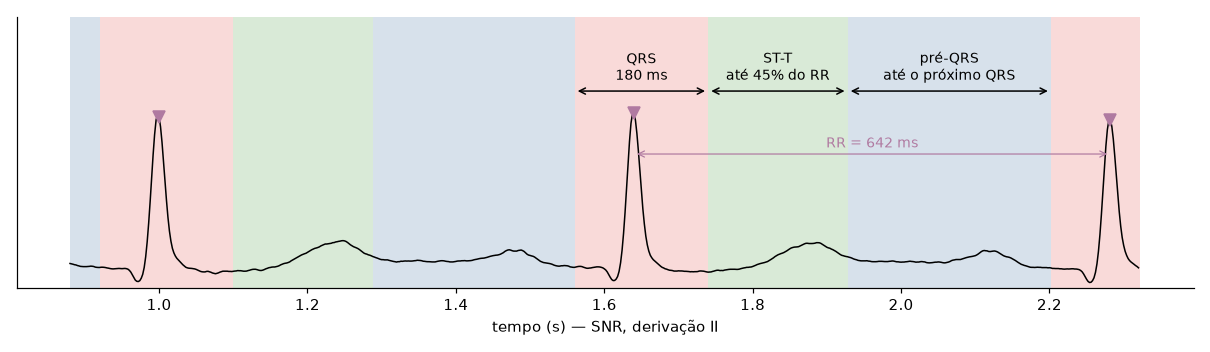
\includegraphics[width=0.9\linewidth]{figs/batimento.png}
\caption{Trecho de cerca de 1,5 s da derivação II de um ECG normal, com três picos R (triângulos) e as regiões de cada batimento: QRS (vermelho), ST‑T (verde) e pré‑QRS (azul). As mesmas regiões são aplicadas às 12 derivações.}
\end{figure}

\textbf{Conferência do código.} (i) A métrica foi calculada antes com um script provisório; os dois, rodados sobre os mesmos mapas, deram resultados idênticos. (ii) O valor esperado ao acaso é obtido por uma fórmula; com as classes embaralhadas entre os mapas 3000 vezes, a média coincidiu com a fórmula.

\subsection{Como os resultados são reportados}
\begin{itemize}
\item \textbf{Consistency crua}, exatamente como definida no artigo (sem ajustes), com o \textbf{valor esperado ao acaso} ao lado apenas como referência.
\item \textbf{Comparação com o F1 descritiva} (ordenação e comparação por classe), sem coeficientes de correlação: as nove classes não são observações independentes (registros multirrótulo, mesmo modelo e mesmo conjunto de teste) nem uma amostra de uma população maior de classes.
\end{itemize}

\section{Achado: a Consistency do Quantus não via os mapas}

Aplicando aos mapas do primeiro treino a mesma normalização, o mesmo valor absoluto e a mesma discretização do Quantus, contou-se quantas explicações simplificadas diferentes existiam em cada classe:

\begin{center}\small
\begin{tabularx}{\linewidth}{Xrrrrrrrr}
\toprule
\textbf{Classe} & SNR & AF & IAVB & BRE & BRD & CAP & STD & STE \\
\midrule
\textbf{Mapas} & 76 & 114 & 64 & 19 & 177 & 19 & 76 & 17 \\
\textbf{Explicações distintas} & 1 & 1 & 1 & 1 & 1 & 1 & 1 & 1 \\
\bottomrule
\end{tabularx}
\end{center}

Todos os mapas ficaram com a mesma explicação, (+, +, +, +, +). Para a métrica, todo mapa era vizinho de todos os outros do lote, e o resultado passava a medir só o quanto a classe top‑1 predita era homogênea dentro de cada classe, sem nenhuma relação com o SHAP. É o caso de ψ “grossa demais” discutido na citação da p. 11. Por isso, aquela versão acompanhava o F1 por razões mecânicas.

\section{Resultados atuais (modelo B)}

O modelo B é o classificador atual: treino alinhado a Zhang et al. (2021), BCE simples e limiares por classe, com F1‑macro de \textbf{0,819} no teste (artigo: 0,813). Foram gerados 622 mapas SHAP, um para cada predição correta do teste. A Consistency global foi \textbf{0,42}, contra 0,13 esperado ao acaso.

\begin{center}\small
\begin{tabularx}{\linewidth}{lrrrrX}
\toprule
\textbf{Classe} & \textbf{Mapas} & \textbf{F1} & \textbf{Consistency} & \textbf{Acaso} & \textbf{Explicação mais comum (k = 2)} \\
\midrule
BRD & 172 & 0,927 & 0,64 & 0,23 & V1·QRS + V2·QRS \\
STD & 65 & 0,778 & 0,51 & 0,09 & II·ST‑T + aVR·ST‑T \\
IAVB & 61 & 0,884 & 0,45 & 0,08 & II·pré‑QRS + aVR·pré‑QRS \\
AF & 108 & 0,931 & 0,42 & 0,14 & V4·QRS + V5·QRS \\
CVP & 59 & 0,837 & 0,26 & 0,08 & aVR·QRS + V5/aVF·QRS \\
BRE & 20 & 0,870 & 0,25 & 0,03 & V1·QRS + V2·QRS \\
SNR & 78 & 0,796 & 0,21 & 0,10 & aVR·pré‑QRS + V1·QRS \\
CAP & 45 & 0,750 & 0,14 & 0,06 & dispersa \\
STE & 14 & 0,596 & 0,03 & 0,02 & pré‑QRS (esperado: ST‑T) \\
\bottomrule
\end{tabularx}
\end{center}

\begin{infobox}[ok]{O que é o valor esperado ao acaso}
É a Consistency que se obteria se as explicações não tivessem nenhuma relação com a classe, como se as classes fossem sorteadas entre os mapas. Nada é descontado: ele serve só como referência. Não é zero porque, mesmo com explicações sorteadas, mapas com a mesma explicação às vezes seriam da mesma classe por coincidência, o que é mais frequente nas classes grandes. Por exemplo, 172 dos 622 mapas são de BRD, e o acaso dessa classe é 0,23; o STE tem 14 mapas, e o acaso dele é 0,02. Assim, BRD (0,64) está bem acima do acaso, e STE (0,03) praticamente nele.
\end{infobox}

\begin{figure}[H]
\centering
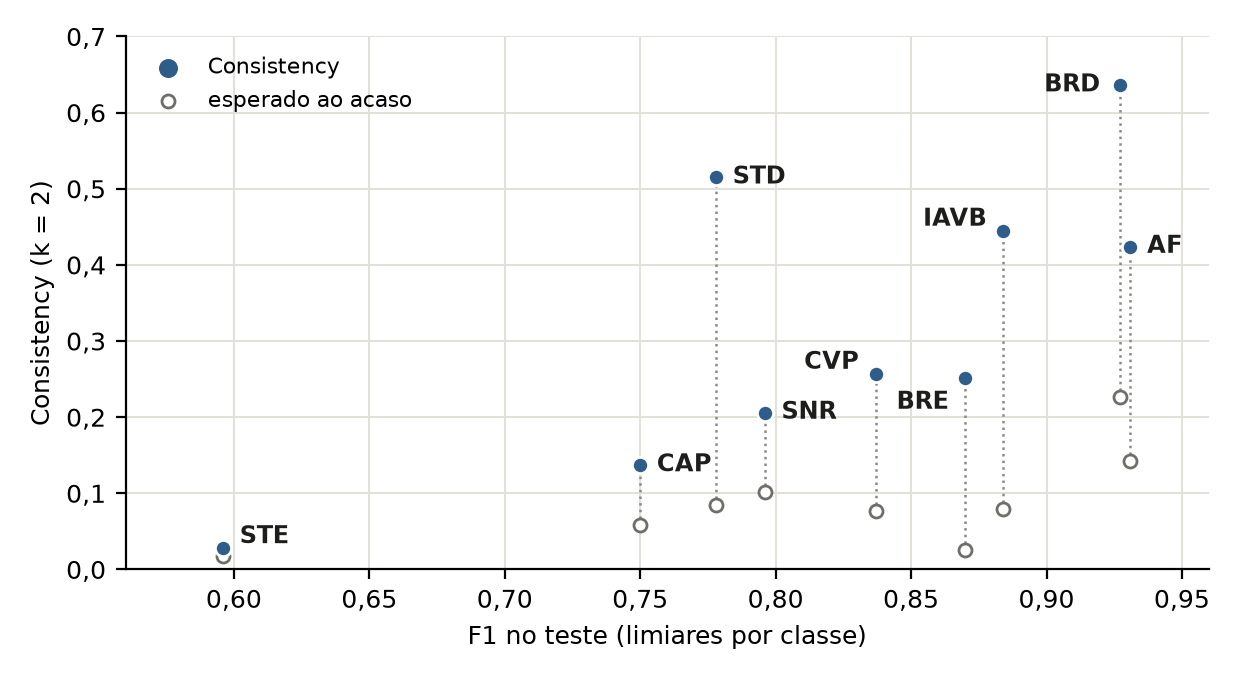
\includegraphics[width=0.7\linewidth]{figs/f1_vs_consistency.png}
\caption{F1 × Consistency por classe (modelo B). Círculos vazios: valor esperado ao acaso; a haste mostra o quanto cada classe fica acima dele.}
\end{figure}

\subsection{Comparação descritiva com o F1}
\begin{center}\small
\begin{tabularx}{\linewidth}{lrrX}
\toprule
\textbf{Classe} & \textbf{Posição no F1} & \textbf{Posição na Consistency} & \textbf{Leitura} \\
\midrule
BRD & 2º & 1º & Concordância no topo \\
IAVB & 3º & 3º & Concordância no topo \\
AF & 1º & 4º & Concordância no topo \\
CVP & 5º & 5º & Posições intermediárias e próximas \\
SNR & 6º & 7º & Posições intermediárias e próximas \\
STD & 7º & 2º & \textbf{Discordância}: F1 intermediário, explicações muito consistentes (ST‑T) \\
BRE & 4º & 6º & \textbf{Discordância}: bom F1, explicações pouco consistentes (20 mapas) \\
CAP & 8º & 8º & Concordância na base \\
STE & 9º & 9º & Concordância na base \\
\bottomrule
\end{tabularx}
\end{center}

As duas ordenações coincidem nas pontas e divergem no meio, com STD e BRE.

\subsection{Sensibilidade às escolhas do método}
O cálculo foi repetido com 9 combinações de regiões (janela do QRS de 140, 180 ou 220 ms × fim do ST‑T em 40, 45 ou 50\% do RR) e com k ∈ \{1, 2, 3\}:

\begin{center}\small
\begin{tabularx}{\linewidth}{lrrX}
\toprule
\textbf{k} & \textbf{Mapas sem par} & \textbf{Consistency global} & \textbf{Observação} \\
\midrule
1 & 1–2\% & 0,40–0,45 & Mais verificável; explicação mais pobre \\
2 & 17–20\% & 0,39–0,45 & Escolha atual; BRD sempre em 1º, CAP e STE sempre nas duas últimas posições \\
3 & 46–50\% & 0,29–0,32 & Metade dos mapas sem par: não verificável \texttt{[p. 11]} \\
\bottomrule
\end{tabularx}
\end{center}

\section{Interpretação e limitações}

\textbf{Conclusões parciais}, só com F1 e Consistency:
\begin{enumerate}
\item As explicações carregam informação sobre a classe, de forma moderada: 0,42 contra 0,13 ao acaso, cerca de 3 vezes o esperado, mas longe de 1.
\item A Consistency é alta onde o diagnóstico depende de um marcador morfológico localizado (BRD, STD, IAVB), e as regiões destacadas coincidem com os critérios clínicos (QRS em V1 no BRD, ST‑T no STD, intervalo PR no IAVB). É plausibilidade, ainda sem validação por especialista.
\item Desempenho e consistência coincidem nas pontas (BRD, IAVB e AF no topo; CAP e STE na base), com exceções no meio (STD e BRE). As duas dimensões andam juntas, mas não se confundem.
\item O padrão depende do modelo: com o classificador anterior (F1 0,641), as posições coincidiam menos (BRE era 3º no F1 e último na Consistency).
\item A discretização determina o resultado da métrica: a versão padrão do Quantus produzia uma coincidência artificial com o F1.
\end{enumerate}

\textbf{Limitações.}
\begin{itemize}
\item \textbf{Populações diferentes} \texttt{[p. 15–16]}: cada classe é uma população com tamanho próprio. Classes pequenas têm valores menos estáveis (STE: 14 mapas) e menor valor esperado ao acaso. A variância do estimador cresce com n pequeno \texttt{[p. 11]}.
\item \textbf{Só acertos}: apenas as predições corretas foram explicadas; não se sabe como as explicações se comportam nos erros.
\item \textbf{Coerência, não correção}: a Consistency mede se explicações iguais levam à mesma classe, e não se a explicação está clinicamente correta.
\item \textbf{Um modelo e uma divisão dos dados}, com 9 classes não independentes: a comparação com o F1 é descritiva.
\end{itemize}

\section{Como redigir no TCC}

\begin{infobox}[ok]{Sugestão: retirada da Sufficiency}
“Dasgupta, Frost e Moshkovitz (2022) propõem duas medidas de fidelidade, consistency e sufficiency. Para métodos de importância de atributos, como o SHAP, os autores não definem quando uma explicação se aplica a outra instância, e por isso analisam apenas a consistency. A implementação de sufficiency da biblioteca Quantus contorna essa lacuna comparando mapas de atribuição por distância, o que equivale a uma consistency relaxada. Por não corresponder à definição original, essa métrica não foi utilizada.”
\end{infobox}

\begin{infobox}[ok]{Sugestão: método da Consistency}
“A consistency foi implementada pelo autor a partir da definição e do estimador de Dasgupta, Frost e Moshkovitz (2022), pois a implementação da biblioteca Quantus (v0.6.0) atribuía a mesma explicação discretizada a todos os mapas avaliados. Cada batimento foi dividido em três regiões (pré-QRS, QRS e ST-T) a partir dos picos R detectados com a biblioteca NeuroKit2, e cada mapa foi resumido pela soma das atribuições por derivação e região. A explicação discretizada consistiu nas duas regiões de maior importância absoluta, com seus sinais. A métrica foi calculada sobre todos os mapas em conjunto, tomando como predição a classe explicada, e é reportada por classe junto do valor esperado ao acaso.”
\end{infobox}

\begin{infobox}[ok]{Sugestão: resultados}
“A consistency global foi de 0,42, frente a 0,13 esperado ao acaso. Os valores mais altos ocorreram em classes com marcador morfológico localizado (BRD, 0,64; STD, 0,51; IAVB, 0,45), cujas regiões mais frequentes coincidem com critérios clínicos, e os mais baixos em STE (0,03) e CAP (0,14). Comparando as ordenações, as classes de melhor e pior desempenho preditivo coincidem com as de maior e menor consistency, com exceções nas posições intermediárias (STD e BRE).”
\end{infobox}

\end{document}
